% =============================================
% =============================================
% Document class: Article
\documentclass[ a4paper, twoside, 11pt]{article}
% Packages: LaTeX (Depth-1)
\usepackage[ vlined, linesnumbered, ruled]{algorithm2e}
\usepackage{ amsfonts, amsmath, amssymb, amsthm}
\usepackage[ titletoc, title]{appendix}
\usepackage{ bbm}
\usepackage{ color}
\usepackage{ dsfont}
\usepackage{ enumitem}
\usepackage{ graphicx}
\usepackage{ fancyhdr, float, fullpage}
\usepackage{ hyperref}
\usepackage{ lastpage, latexsym, lipsum}
\usepackage{ mathrsfs, mathtools, multicol}
\usepackage{ parskip}
\usepackage{ setspace, stmaryrd, subcaption}
\usepackage{ tabularx}
\usepackage{ wasysym}
\usepackage[ dvipsnames, table]{ xcolor}
\usepackage{ xfrac}
% Packages: LaTeX (Depth-2)
\usepackage{ epstopdf}

% =============================================
\topmargin 			= -1.6cm
\headheight 		= .90cm
\headsep 			= .80cm
\textheight 		= 24.0cm
\textwidth 			= 15.5cm
\oddsidemargin		= 0.cm
\evensidemargin 	= 0.cm

% =============================================
% =============================================
% Macros: Language
\newcommand{\define}{\triangleq}
\newcommand{\done}{\hfill $\square$}
%\newcommand{\eqCIRC}{\stackrel{\circ}{=}}
%\newcommand{\eqSTAR}{\stackrel{*}{=}}
\renewcommand{\epsilon}{\varepsilon}
\newcommand{\eg}{\textit{e.g.,\;}}
\newcommand{\egc}{\textit{e.g.:\;}}
\newcommand{\Eg}{\textit{E.g.,\;}}
\newcommand{\Egc}{\textit{E.g.:\;}}
\newcommand{\ie}{\textit{i.e.,\;}}
\newcommand{\iec}{\textit{i.e.:\;}}
\newcommand{\Ie}{\textit{I.e.,\;}}
\newcommand{\Iec}{\textit{I.e.:\;}}
\newcommand{\QED}{\hfill $\blacksquare$}
\renewcommand{\tilde}[1]{\widetilde{#1}}
\newcommand{\tsup}[1]{\ensuremath{^{\text{#1}}}}
\newcommand{\tsub}[1]{\ensuremath{_{\text{#1}}}}
\renewcommand{\vec}[1]{{\boldsymbol{#1}}}

% Macros: Optimization & Probability
\DeclareMathOperator*{\argmax}{arg\,max}
\DeclareMathOperator*{\argmin}{arg\,min}
\newcommand{\Exp}{\mathbb{E}}
\newcommand{\Indicate}[1]{ \IndFun \, \{ \, #1 \, \} }
\renewcommand{\Pr}{\mathbb{P}}
\newcommand{\Normal}{\mathcal{N}}
\newcommand{\std}{\text{std}}
\newcommand{\var}{\text{var}}

% Macros: Sets
\newcommand{\Complex}{\mathbb{C}}
\renewcommand{\emptyset}{\varnothing}
\newcommand{\Nat}{\mathbb{N}}
\renewcommand{\Re}{\mathbb{R}}
\newcommand{\ReNN}{{\Re}_{\geq 0}}
\newcommand{\ReSP}{{\Re}_{> 0}}
\renewcommand{\subset}{\subseteq}
\renewcommand{\supset}{\supseteq}
\newcommand{\Z}{\mathbb{Z}}
\newcommand{\ZNN}{{\Z}_{\geq 0}}

% Macros: Spacing & Other Commands
\newcommand{\fullcut}{\vspace{-\baselineskip}}
\newcommand{\fullskip}{\vspace{\baselineskip}}
\newcommand{\halfcut}{\vspace{-0.5\baselineskip}}
\newcommand{\halfskip}{\vspace{0.5\baselineskip}}
\renewcommand{\figurename}{Figura}
\renewcommand{\tablename}{Tabla}

% =============================================
% Sesion de Clase
\newcommand{\sesion}{03}
% Macros para definiciones, teoremas, etc
\newcounter{sesion}
\setcounter{sesion}{\sesion}
\theoremstyle{definition}
\newtheorem{definition}{Definici\'on}[sesion]
\newtheorem{example}[definition]{Ejemplo}
\newtheorem{exercise}[definition]{Ejercicio}
\newtheorem{note}[definition]{Nota}
\newtheorem{problem}[definition]{Problema}
\newtheorem{theorem}[definition]{Teorema}

% =============================================
% =============================================
\newcommand{\HeaderLine}{}
\newcommand{\FooterLine}{P\'agina \thepage ~de \pageref*{LastPage}}

\pagestyle{fancyplain}
\fancyhf{}

\rhead[]{\fancyplain{}{\HeaderLine}}
\lhead[\fancyplain{}{\HeaderLine}]{}
\lfoot[\fancyplain{}{\FooterLine}]{}
\rfoot[]{\fancyplain{}{\FooterLine}}

\renewcommand{\headrulewidth}{0.4pt}
\renewcommand{\footrulewidth}{0.4pt}
\renewcommand{\thefootnote}{\fnsymbol{footnote}}

% =============================================
% =============================================
\begin{document}
\allowdisplaybreaks

\begin{center}
\Large Control Autom\'atico: Lecci\'on \sesion \\[0.5ex]
\small \textbf{A\~no:} 2016-2017 \qquad \textbf{T\'ermino:} II \qquad
\textbf{Instructor:} Luis I. Reyes Castro \qquad \textbf{Paralelo:} 02
\end{center}
\halfskip

\fbox{

\begin{minipage}[b][\height][t]{\textwidth}
\vspace{0.2 cm}

\begin{center}
\textbf{COMPROMISO DE HONOR}
\end{center}
\vspace{0.4 cm}

\scriptsize
{
Yo, \rule{60mm}{.1pt} al firmar este compromiso, reconozco que la presente lecci\'on est\'a dise\~nada para ser resuelta de manera individual, que puedo usar un l\'apiz o pluma y una calculadora cient\'ifica, \linebreak que solo puedo comunicarme con la persona responsable de la recepci\'on de la lecci\'on, y que cualquier instrumento de comunicaci\'on que hubiere tra\'ido debo apagarlo. Tambi\'en estoy conciente que no debo consultar libros, notas, \linebreak ni materiales did\'acticos adicionales a los que el instructor entregue durante la lecci\'on o autorice a utilizar. Finalmente, me comprometo a desarrollar y presentar mis respuestas de manera clara y ordenada. \\

Firmo al pie del presente compromiso como constancia de haberlo le\'ido y aceptado. 
\vspace{0.4 cm}

Firma: \rule{60mm}{.1pt} \qquad N\'umero de matr\'icula: \rule{40mm}{.1pt} \hspace{0.5cm} \\[-0.8ex]

}

\end{minipage}

}
\vspace{\baselineskip}

% =============================================
\begin{problem}
\textbf{[5 Puntos]} Considere el siguente modelo de un tren urbano el\'ectrico de cuatro vagones. Los vagones 1 y 4 son vagones-locomotoras que producen las fuerzas $F_1(t)$ y $F_4(t)$ que empujan el tren. 
\begin{figure}[htb]
\centering
\def\svgwidth{0.8\columnwidth}
\input{leccion_03_prob_tren.eps_tex}
\end{figure}

Suponiendo por simplicidad que la fuerza de arrastre aerodin\'amico $F_{aero}(t)$ act\'ua solamente sobre el vag\'on 1 y que esta fuerza tiene una magnitud proporcional a la velocidad promedio de todos los vagones del tren (donde la constante de proporcionalidad es $K_{aero}$), construya un modelo de espacio de estados con las siguientes caracteristicas: 
\begin{itemize}
\item Las entradas son las fuerzas de los vagones-locomotoras, \ie la primera entrada es $F_1(t)$ y la segunda entrada es $F_4(t)$. 
\item Las salidas son las velocidades relativas de los vagones, \ie la primera salida es la velocidad del vag\'on 1 relativa al vag\'on 2, la segunda salida es la velocidad del vag\'on 2 relativa al vag\'on 3, y la tercera salida es la velocidad del vag\'on 3 relativa al vag\'on 4. 
\item Todos los estados asociados con el vag\'on 1 se listan antes de los estados asociados con el vag\'on 2, los cuales se listan antes de los estados asociados con el vag\'on 3, y asi sucesivamente. Adem\'as, los estados asociados con posiciones se listan antes que los estados asociados con velocidades. 
\end{itemize}

\emph{Soluci\'on:} Primero, como el sistema tiene 4 bloques de masa lo modelamos con 8 estados, donde para cada bloque $i \in \{ 1, \dots, 4 \}$ las variables de estado $x_i(t)$ y $v_i(t)$ denotan la posici\'on y velocidad del bloque, respectivamente. Luego, escribimos las cuatro ecuaciones diferenciales asociadas con los vagones (\ie bloques de masa): 
\begin{itemize}
\item En el vag\'on 1: 
\begin{align*}
\left( \frac{3}{2} \right) M \, \ddot{x}_1(t) \; 
& = \; F_1(t) - K_{aero} \left( \frac{\dot{x}_1(t) + \dot{x}_2(t) + \dot{x}_3(t) + \dot{x}_4(t)}{4} \right) \\
& - K_s \, ( \, x_1(t) - x_2(t) \, ) - K_d \, ( \, \dot{x}_1(t) - \dot{x}_2(t) \, )
\end{align*}
\item En el vag\'on 2: 
\begin{align*}
M \, \ddot{x}_2(t) \; 
& = \; K_s \, ( \, x_1(t) - x_2(t) \, ) + K_d \, ( \, \dot{x}_1(t) - \dot{x}_2(t) \, ) \\
& - K_s \, ( \, x_2(t) - x_3(t) \, ) - K_d \, ( \, \dot{x}_2(t) - \dot{x}_3(t) \, )
\end{align*}
\item En el vag\'on 3: 
\begin{align*}
M \, \ddot{x}_3(t) \; 
& = \; K_s \, ( \, x_2(t) - x_3(t) \, ) + K_d \, ( \, \dot{x}_2(t) - \dot{x}_3(t) \, ) \\
& - K_s \, ( \, x_3(t) - x_4(t) \, ) - K_d \, ( \, \dot{x}_3(t) - \dot{x}_4(t) \, )
\end{align*}
\item En el vag\'on 4: 
\begin{align*}
\left( \frac{3}{2} \right) M \, \ddot{x}_4(t) \; 
& = \; F_4(t) + K_s \, ( \, x_3(t) - x_4(t) \, ) + K_d \, ( \, \dot{x}_3(t) - \dot{x}_4(t) \, )
\end{align*}
\end{itemize}
Con esto en mente observamos que si los vectores de estado y entrada son 
\[
\vec{x}(t) \; = \; 
\left[ \begin{array}{c}
x_1(t) \\ v_1(t) \\
x_2(t) \\ v_2(t) \\
x_3(t) \\ v_3(t) \\
x_4(t) \\ v_4(t)
\end{array} \right] \qquad \qquad
\vec{u}(t) \; = \; 
\left[ \begin{array}{c} F_1(t) \\ F_4(t) \end{array} \right]
\]
entonces las matrices de estado y de entrada son: 
\[
\vec{A} \; = \; 
\left[ \begin{array}{cc|cc|cc|cc}
0 & 1 & 0 & 0 & 0 & 0 & 0 & 0 \\[1ex]
-\frac{2 K_s}{3 M} & -\frac{2 K_d}{3 M} -\frac{K_{aero}}{6M} & \frac{2 K_s}{3 M} & \frac{2 K_d}{3 M} -\frac{K_{aero}}{6M} & 0 & -\frac{K_{aero}}{6 M} & 0 & -\frac{K_{aero}}{6 M} \\[1ex] \hline
0 & 0 & 0 & 1 & 0 & 0 & 0 & 0 \\[1ex]
\frac{K_s}{M} & \frac{K_d}{M} & -\frac{2 K_s}{M} & -\frac{2 K_d}{M} & \frac{K_s}{M} & \frac{K_d}{M} & 0 & 0 \\[1ex] \hline
0 & 0 & 0 & 0 & 0 & 1 & 0 & 0 \\[1ex]
0 & 0 & \frac{K_s}{M} & \frac{K_d}{M} & -\frac{2 K_s}{M} & -\frac{2 K_d}{M} & \frac{K_s}{M} & \frac{K_d}{M} \\[1ex] \hline
0 & 0 & 0 & 0 & 0 & 0 & 0 & 1 \\[1ex]
0 & 0 & 0 & 0 & \frac{2 K_s}{3 M} & \frac{2 K_d}{3 M} & -\frac{2 K_s}{3M} & -\frac{2 K_d}{3M}
\end{array} \right]
\]
\[
\vec{B} \; = \; 
\left[ \begin{array}{c|c}
0 & 0 \\[1ex]
\frac{2}{3M} & 0 \\[1ex] \hline
0 & 0 \\[1ex]
0 & 0 \\[1ex] \hline
0 & 0 \\[1ex]
0 & 0 \\[1ex] \hline
0 & 0 \\[1ex]
0 & \frac{2}{3M}
\end{array} \right]
\]

Finalmente, recordando la definici\'on de velocidad relativa, vemos que las matrices de salida y de alimentaci\'on delantera son: 
\[
\vec{C} \; = \; 
\left[ \begin{array}{cc|cc|cc|cc}
0 & 1 & 0 & -1 & 0 & 0 & 0 & 0 \\ \hline
0 & 0 & 0 & 1 & 0 & -1 & 0 & 0 \\ \hline
0 & 0 & 0 & 0 & 0 & 1 & 0 & -1
\end{array} \right] \qquad \qquad 
\vec{D} \; = \; 
\left[ \begin{array}{c|c}
0 & 0 \\ \hline 0 & 0 \\ \hline 0 & 0
\end{array} \right]
\]

\end{problem}
\vspace{\baselineskip}

% =============================================
\begin{problem}
\textbf{[5 Puntos]} Considere el siguente circuito anal\'ogico.  
\begin{figure}[htb]
\centering
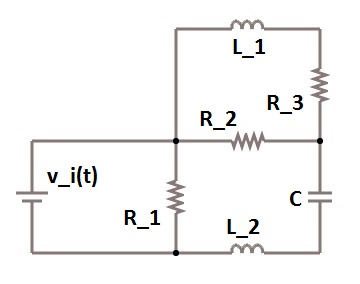
\includegraphics[ width = 0.35\textwidth]{leccion_03_prob_electrico.jpg}
\end{figure}

Construya un modelo de espacio de estados con las siguientes caracter\'isticas: 
\begin{itemize}
\item La entrada es el voltage en la fuente $v_i(t)$. 
\item La salida es el voltage a trav\'es de la resistencia $R_2$. 
\item Todos los estados asociados con corrientes deber\'an ser listados antes de los estados asociados con voltages. 
\end{itemize}

\emph{Soluci\'on:} Primero vemos que el sistema tiene tres elementos capaces de almacenar energ\'ia: el inductor $L_1$, el inductor $L_2$ y el capacitor $C$. Por lo tanto, los estados son: 
\begin{itemize}
\item La corriente a trav\'es del inductor $L_1$, denotada $i_1(t)$. 
\item La corriente a trav\'es del inductor $L_2$, denotada $i_2(t)$. 
\item El voltaje a trav\'es del capacitor $C$, denotado $v_C(t)$. 
\end{itemize}

Luego, por conveniencia introducimos las dos siguientes corrientes, tal como se muestra en la figura de la siguiente p\'agina. 
\begin{itemize}
\item La corriente a trav\'es de la resistencia $R_2$, denotada $i_3(t)$. N\'otese que: 
\[
i_3(t) \; = \; i_2(t) - i_1(t)
\]
\item La corriente a trav\'es de la resistencia $R_1$, denotada $i_4(t)$. N\'otese que: 
\[
i_4(t) \; = \; \frac{v(t)}{R_1}
\]
\end{itemize}
\begin{figure}[htb]
\centering
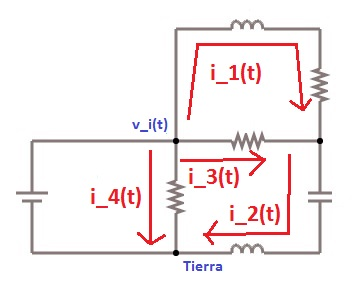
\includegraphics[ width = 0.35\textwidth]{leccion_03_prob_electrico_solucion.jpg}
\end{figure}

Ahora escribimos la ecuaci\'on de estado del inductor $L_1$ : 
\begin{align*}
L_1 \, \frac{di_1(t)}{dt} \; = \; v_{L_1}(t) \; 
& = \; v_{R_2}(t) - v_{R_3}(t) \\
& = \; R_2 \, i_3(t) - R_3 \, i_1(t) \\
& = \; R_2 \, ( \, i_2(t) - i_1(t) \, ) - R_3 \, i_1(t) \; = \; 
- ( \, R_2 + R_3 \, ) \, i_1(t) + R_2 \, i_2(t)
\end{align*}
Luego escribimos la ecuaci\'on de estado del inductor $L_2$ : 
\begin{align*}
L_2 \, \frac{di_2(t)}{dt} \; = \; v_{L_2}(t) \; 
& = \; v_i(t) - v_{R_2}(t) - v_C(t) \\
& = \; v_i(t) - R_2 \, i_3(t) - v_C(t) \\
& = \; v_i(t) - R_2 \, ( \, i_2(t) - i_1(t) \, ) - v_C(t) \\
& = \; R_2 \, i_1(t) - R_2 \, i_2(t) - v_C(t) + v_i(t)
\end{align*}
Despues escribimos la ecuaci\'on de estado del capacitor $C$, la cual resulta ser trivial: 
\[
C \, \frac{dv_C(t)}{dt} \; = \; i_C(t) \; = \; i_2(t)
\]
Con esto en mente observamos que si los vectores de estado y entrada son 
\[
\vec{x}(t) \; = \; 
\left[ \begin{array}{c}
i_1(t) \\ i_2(t) \\ v_C(t)
\end{array} \right] \qquad \qquad
\vec{u}(t) \; = \; 
\left[ \begin{array}{c} v_i(t) \end{array} \right]
\]
entonces las matrices de estado y de entrada son: 
\[
\vec{A} \; = \; 
\left[ \begin{array}{ccc}
-\frac{R_2 + R_3}{L_1} & \frac{R_2}{L_1} & 0 \\[1ex]
\frac{R_2}{L_2} & -\frac{R_2}{L_2} & -\frac{1}{L_2} \\[1ex]
0 & \frac{1}{C} & 0
\end{array} \right] \qquad \qquad
\vec{B} \; = \; 
\left[ \begin{array}{c}
0 \\[1ex] \frac{1}{L_2} \\[1ex] 0
\end{array} \right]
\]

Finalmente, dado que la salida es el voltaje a traves de la resistencia $R_2$, tenemos que: 
\[
v_{R_2}(t) \; = \; R_2 \, i_3(t) \; = \; R_2 \, ( \, i_2(t) - i_1(t) \, ) \; = \; -R_2 \, i_1(t) + R_2 \, i_2(t)
\]
Consecuentemente las matrices de salida y de alimentaci\'on delantera son: 
\[
\vec{C} \; = \; 
\left[ \begin{array}{ccc}
-R_2 & R_2 & 0
\end{array} \right] \qquad \qquad
\vec{D} \; = \; 
\left[ \begin{array}{c} 0 \end{array} \right]
\]

\end{problem}
\vspace{\baselineskip}

\end{document}
